\chapter{Diseños individuales para la iteración competitiva de Alberto Alejandro Rivas Fernandez}
\label{ape:disenyoAlberto}

En este apéndice se muestran los diseños individuales realizados por Alberto Alejandro Rivas Fernández para la iteración competitiva.

En primer lugar, en la Figura \ref{AlbertoPaginaPrincipal1} se muestra la página principal antes de haber seleccionado un documento PDF, por lo que hay un elemento en el que podemos subir un fichero. Luego en la Figura \ref{AlbertoPaginaPrincipal2}  tenemos la página principal después de haber seleccionado un documento, en la parte izquierda se muestra dicho documento y en la parte derecha tenemos el editor de texto con todos los botones para acceder a las funcionalidades en la parte superior. 

En la Figura \ref{Alberto13} se muestra el ejercicio de huecos, en el que el usuario puede escribir un texto y seleccionar qué palabras quiere sustituir por un hueco. En la Figura \ref{Alberto14} se observa el ejercicio de definiciones, en el que el usuario puede añadir una serie de definiciones e indicar la cantidad de líneas que quiere insertar para cada definición, junto con otras opciones. En la Figura \ref{Alberto15} está el ejercicio de desarrollo, que consta de un área de texto en la que se puede escribir el enunciado del ejercicio, también se puede indicar la cantidad de líneas junto con otras opciones. En la Figura \ref{Alberto16} se presenta el ejercicio de sopa de letras, que permite ajustar el tamaño, las direcciones, etc. En la Figura \ref{Alberto17} se encuentra el ejercicio de verdadero y falso, en el que el usuario puede añadir una serie de frases. En la Figura \ref{Alberto1} se muestra la leyenda de colores, que permite añadir una serie de frases acompañadas de un color. En la Figura \ref{Alberto2} se observa la leyenda de colores por asignatura, que permite añadir un borde de color a la página, el cual indica la asignatura a la que pertenece. En las Figuras \ref{Alberto3} y \ref{Alberto4} se encuentran los modales para insertar cuadrículas y líneas de doble pauta. En la Figura \ref{Alberto5} se encuentra el ejercicio de flechas, el cual tiene dos columnas donde el usuario puede escribir los conceptos a relacionar. En la Figura \ref{Alberto6} se muestra el ejercicio de matemática con huecos, en el que se puede escribir una fórmula con LaTeX. En las Figuras \ref{Alberto8} y \ref{Alberto10} se observan los modales de generar resumen y pictotraductor, en los cuales se inserta un texto y se resume o traduce a pictogramas respectivamente. En la Figura \ref{Alberto7} se presenta el modal de espacio para dibujar, en el que se puede indicar la altura y anchura que tendrá el espacio. Por último, en la Figura \ref{Alberto12} se encuentra el buscador de pictogramas, que consta de una barra de búsqueda y los resultados mostrados en forma de cuadrícula.



\begin{figure}[ht!]
  \centering
  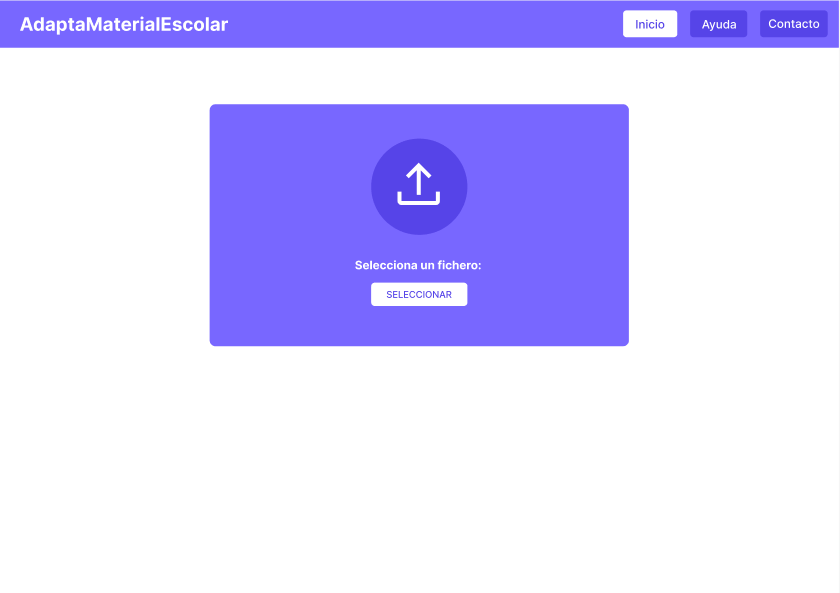
\includegraphics[width=0.6\textwidth]{Diseño/Alberto/PaginaPrincipal1.PNG}
  \caption{Diseño página principal de Alberto.}
  \label{AlbertoPaginaPrincipal1}
\end{figure}

\begin{figure}[ht!]
  \centering
  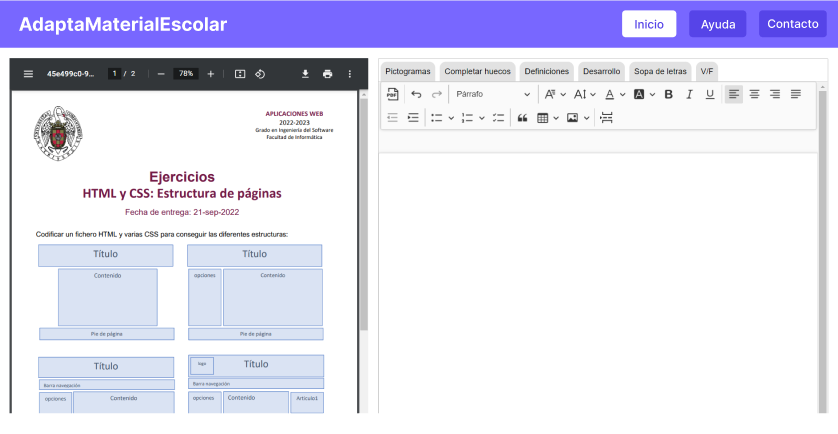
\includegraphics[width=0.6\textwidth]{Diseño/Alberto/PaginaPrincipal2.PNG}
  \caption{Diseño página principal de Alberto.}
  \label{AlbertoPaginaPrincipal2}
\end{figure}


\begin{figure}[ht!]
  \centering
  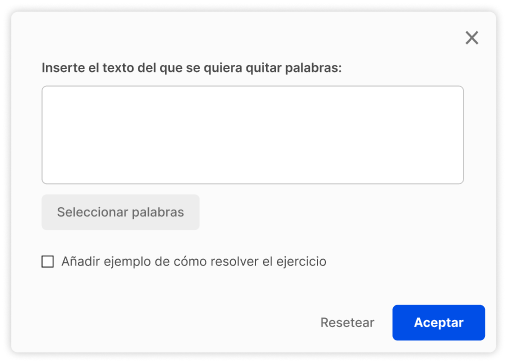
\includegraphics[width=0.6\textwidth]{Diseño/Alberto/Capture13.PNG}
  \caption{Diseño de ejercicios con huecos de Alberto.}
  \label{Alberto13}
\end{figure}

\begin{figure}[ht!]
  \centering
  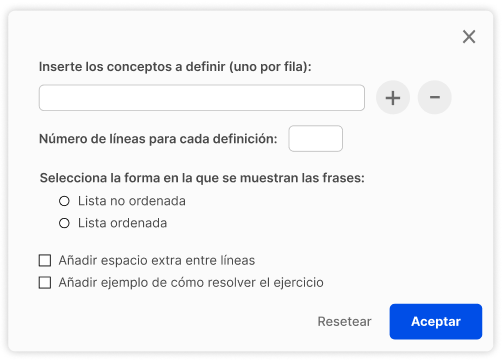
\includegraphics[width=0.6\textwidth]{Diseño/Alberto/Capture14.PNG}
  \caption{Diseño de ejercicios de definiciones de Alberto.}
  \label{Alberto14}
\end{figure}

\begin{figure}[ht!]
  \centering
  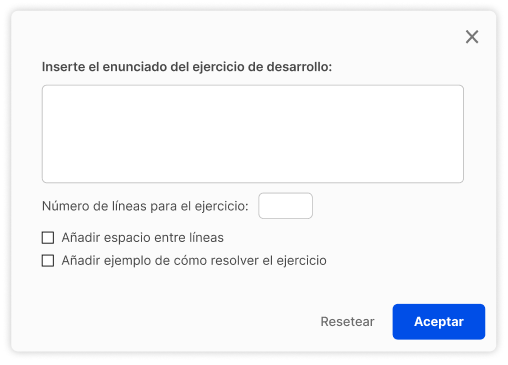
\includegraphics[width=0.6\textwidth]{Diseño/Alberto/Capture15.PNG}
  \caption{Diseño de ejercicios de desarrollo de Alberto.}
  \label{Alberto15}
\end{figure}

\begin{figure}[ht!]
  \centering
  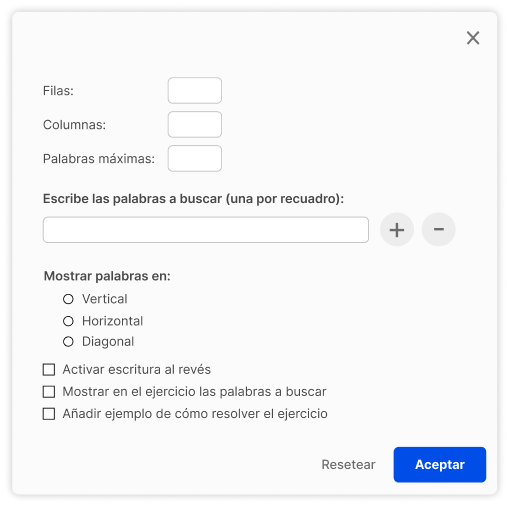
\includegraphics[width=0.6\textwidth]{Diseño/Alberto/Capture16.PNG}
  \caption{Diseño de ejercicios de sopa de letras de Alberto.}
  \label{Alberto16}
\end{figure}

\begin{figure}[ht!]
  \centering
  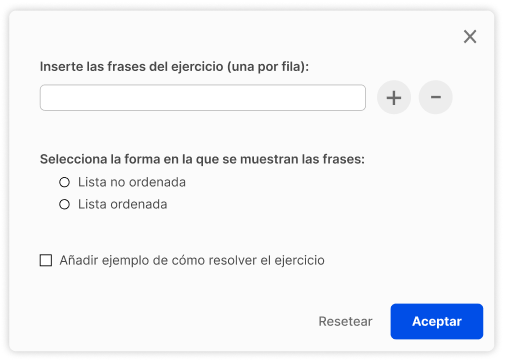
\includegraphics[width=0.6\textwidth]{Diseño/Alberto/Capture17.PNG}
  \caption{Diseño de ejercicios de verdadero y falso de Alberto.}
  \label{Alberto17}
\end{figure}


\begin{figure}[ht!]
  \centering
  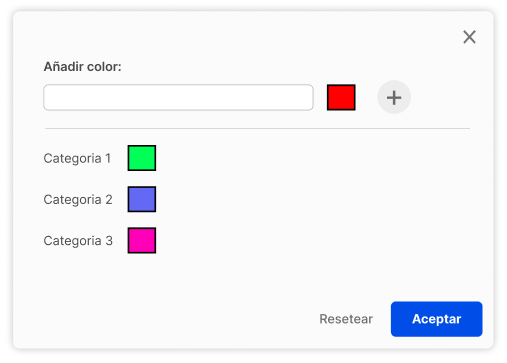
\includegraphics[width=0.6\textwidth]{Diseño/Alberto/Capture01.PNG}
  \caption{Diseño de leyenda de colores de Alberto.}
  \label{Alberto1}
\end{figure}

\begin{figure}[ht!]
  \centering
  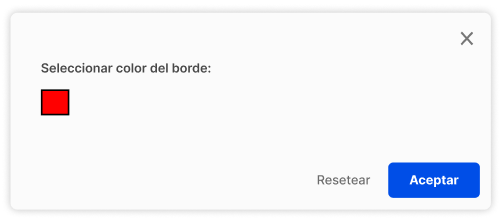
\includegraphics[width=0.6\textwidth]{Diseño/Alberto/Capture02.PNG}
  \caption{Diseño de leyenda de colores por asignatura de Alberto.}
  \label{Alberto2}
\end{figure}

\begin{figure}[ht!]
  \centering
  
\includegraphics[width=0.6\textwidth]{Diseño/Alberto/Capture03.PNG}
  \caption{Diseño de cuadrícula de Alberto.}
  \label{Alberto3}
\end{figure}

\begin{figure}[ht!]
  \centering
  
\includegraphics[width=0.6\textwidth]{Diseño/Alberto/Capture04.PNG}
  \caption{Diseño de doble pauta de Alberto.}
  \label{Alberto4}
\end{figure}

\begin{figure}[ht!]
  \centering
  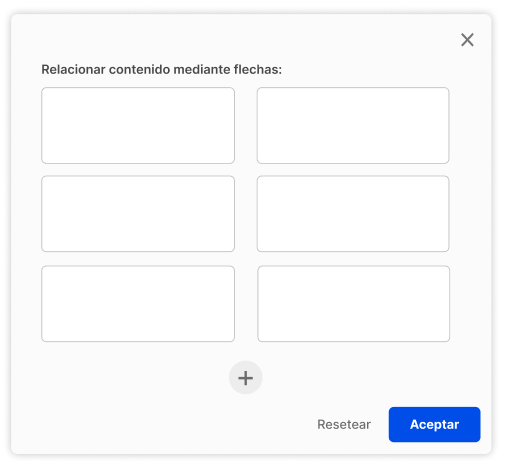
\includegraphics[width=0.6\textwidth]{Diseño/Alberto/Capture05.PNG}
  \caption{Diseño de ejercicio de flechas de Alberto.}
  \label{Alberto5}
\end{figure}

\begin{figure}[ht!]
  \centering
  
\includegraphics[width=0.6\textwidth]{Diseño/Alberto/Capture06.PNG}
  \caption{Diseño de ejercicios de matemáticas con huecos de Alberto.}
  \label{Alberto6}
\end{figure}

\begin{figure}[ht!]
  \centering
  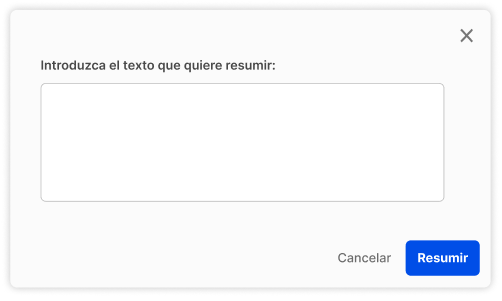
\includegraphics[width=0.6\textwidth]{Diseño/Alberto/Capture08.PNG}
  \caption{Diseño de añadir resumen de Alberto.}
  \label{Alberto8}
\end{figure}

\begin{figure}[ht!]
  \centering
  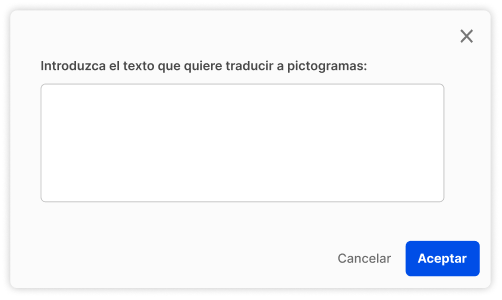
\includegraphics[width=0.6\textwidth]{Diseño/Alberto/Capture10.PNG}
  \caption{Diseño de pictotraductor de Alberto.}
  \label{Alberto10}
\end{figure}

\begin{figure}[ht!]
  \centering
  
\includegraphics[width=0.6\textwidth]{Diseño/Alberto/Capture07.PNG}
  \caption{Diseño de ejercicios de espacios para dibujar de Alberto.}
  \label{Alberto7}
\end{figure}

\begin{figure}[ht!]
  \centering
  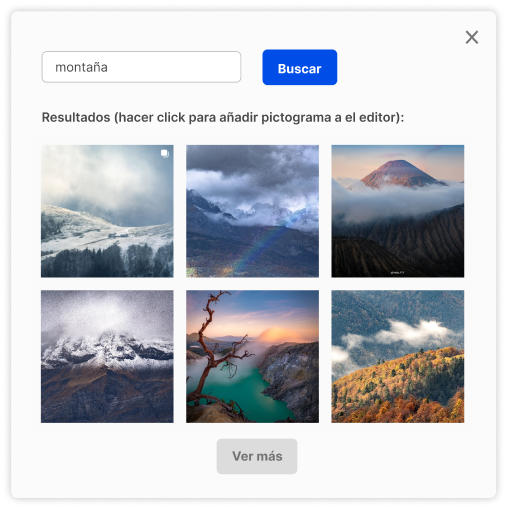
\includegraphics[width=0.6\textwidth]{Diseño/Alberto/Capture12.PNG}
  \caption{Diseño de buscar pictogramas de Alberto.}
  \label{Alberto12}
\end{figure}